% !TeX spellcheck = en_GB
% !TeX root = Report.tex
\phantomsection
\addcontentsline{toc}{section}{Introduction}
\sect{Introduction}

Government legislation pervades all aspects of modern life from welfare to industry, infrastructure to enterprise.
This report is primarily concerned with legislation that governs industry and the pertaining profit potential.
The dictionary definition of legislation is ``laws, considered collectively'' \cite{OED} and the two terms are used synonymously in this report.
One of the main roles of the elected parliament is the debate and passing of new laws or modification to laws.


\begin{figure}[!h]
\centering
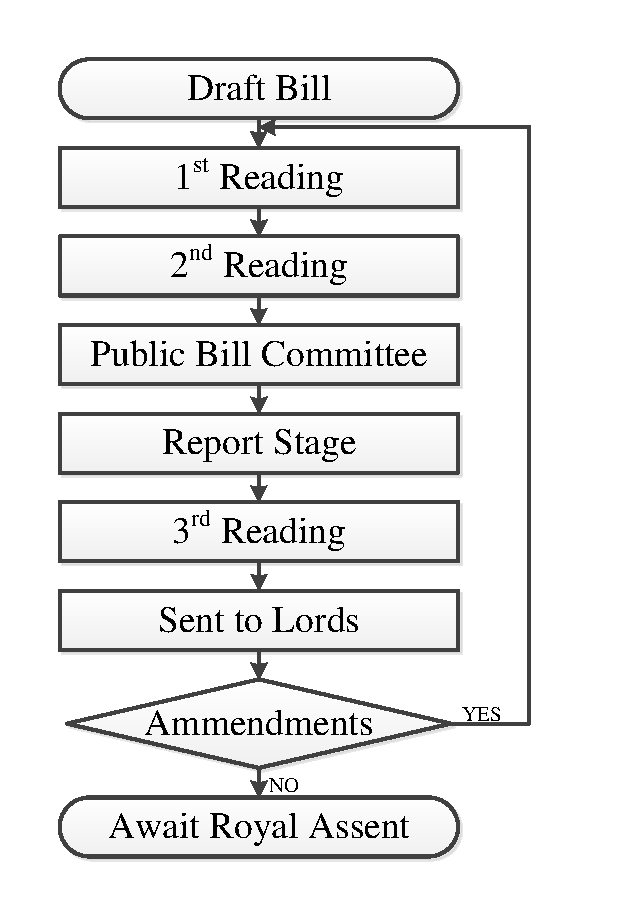
\includegraphics[width = 0.3\textwidth]{Figures/BillFormulation.pdf}
\caption{The passage of a Bill or Act to become Law}
\label{figure:passage}
\end{figure}


